\documentclass[onecolumn]{article}
\usepackage[utf8]{inputenc}
\usepackage{graphicx}
\usepackage[cmex10]{amsmath}
\usepackage[spanish]{babel}
\usepackage{mdframed}
\usepackage{url}

\renewcommand{\thesubsection}{\thesection.\arabic{subsection}}

%opening
\title{TP2 - Sistemas de información geográfica en la gestión de EAPs}
\author{Guillermo Federico Olmedo}


\begin{document}
\markboth{Curso de Zonificación Vitícola y Viticultura de precisión - 2016}{}

\maketitle

\tableofcontents
\bigskip

\textbf{Los archivos necesarios para completar este trabajo práctico se encuentran en la carpeta de “Datos/TP2”. }\\

\begin{mdframed}
	Para completar con éxito este ejercicio, debe escribir un informe con las respuestas a las preguntas que aparecen en cajas como esta. El informe debe remitirse en formato pdf por correo electrónico a: \url{olmedo.guillermo@inta.gob.ar}
\end{mdframed}


\section{La interfaz de QGIS}

\subsection{Creando nuestro proyecto de trabajo}

Cuando iniciamos el programa, por defecto se comienza con un proyecto nominado “sin titulo”.

\begin{figure}
\centering
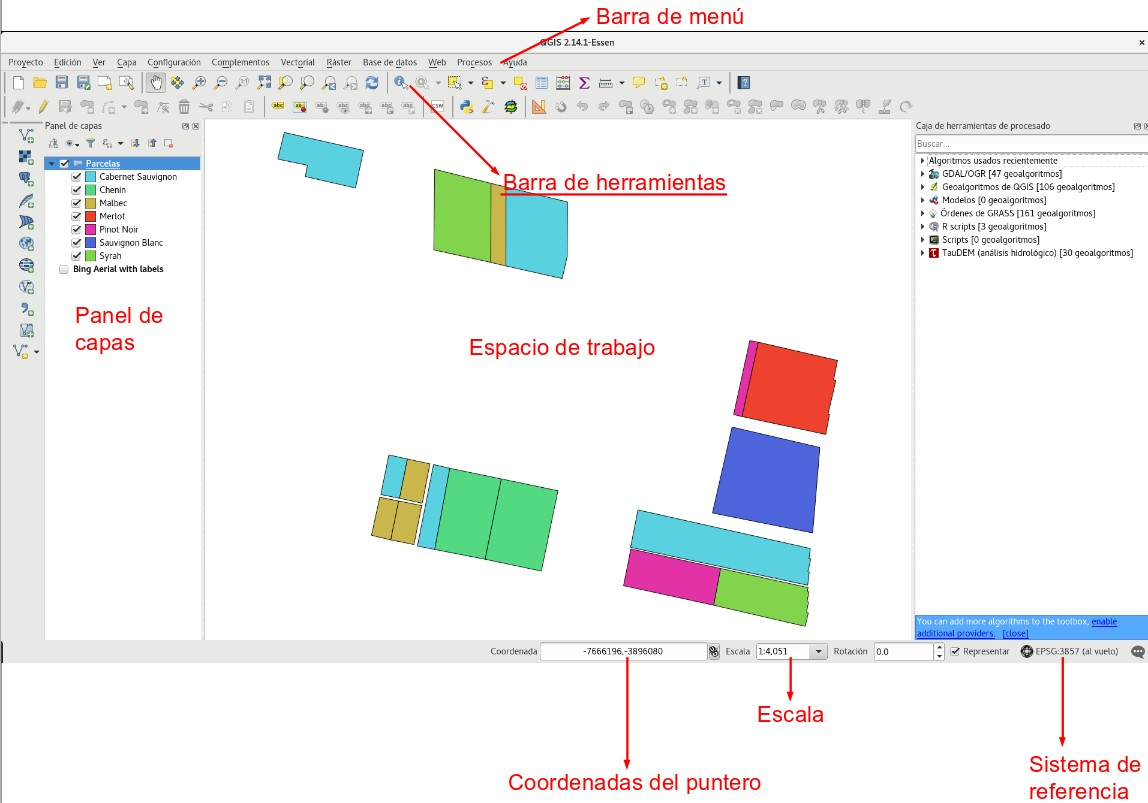
\includegraphics[width=1\linewidth]{IMGs/interfaz}
\caption{La interfaz de QGIS}
\label{fig:interfaz}
\end{figure}


El proyecto se puede guardar desde la barra de menús: “Archivo -----> Guardar Proyecto Como”, a través del atajo de teclado Ctrl+G, o cuando salgamos del programa respondiendo a la ventana de seguridad que se abre al intentar cerrar el programa. 
Este proyecto guardará la lista de capas que se encuentren cargadas en nuestra Tabla de Contenidos, su respectivas paletas de color y la ultima vista del Espacio de Trabajo.\\

Vamos a establecer además el sistema de coordendas para nuestro proyecto en Posgar 94 faja 2, (Posgar 94 / Argentina 2; EPSG 22182) y activar la transformación de SRC al vuelo haciendo click en el ícono del mundo en la esquina inferior izquierda de la interfaz de QGIS. 
Al presionar este botón se desplegará un diálogo que nos permitirá elegir el sistema de coordendas\footnote{Puede usar el campo filtrar para encontrar más rapidamente el sistema de coordendas.}. Recuerde activar la transformación de SRC al vuelo.\\


%%%%%%%%%%%%%%%%%%%%%%%%%%%%%%%%%%%%

\begin{mdframed}[]
	Pregunta 1: Que código corresponde al SRC Campo Inchauspe / Argentina 2? Mire el código proj4, compárelo con EPSG:22172. Utilizan el mismo geoide? En que unidades están ambos sistemas? Y en que unidades está EPSG:4456
\end{mdframed}



\subsection{Agregando capas raster a nuestro entorno de trabajo}

Dentro de las Barras de herramientas mostradas por defecto en el entorno QGIS, se encuentra la barra de administrar capas, a través de ella se cargan al entorno de trabajo las capas vectoriales, raster, etc. (vea los iconos detallados en la presentación).


\begin{center}
	\includegraphics[width=0.5\linewidth]{IMGs/agregar}
\end{center}

Agregamos la capa de tipo raster (pulsando el ícono remarcado)\footnote{Al dejar el puntero del mouse detenido sobre los iconos, se despliega en estos una breve descripción de los mismos.}, QB\_Finca.tif que utilizaremos como mapa base.\\

Modificando las propiedades de la capa:

Cuando se carga una capa raster al espacio de trabajo de QGIS, en el general de los casos esta se verá de color gris uniforme. 
Esto sucede debido a que el programa grafica los datos según una paleta estándar en la gama de los grises, y cuyo rango es generalmente mucho mas grande que el de las imágenes. 
Para modificar la representación es necesario ingresar a la capa de atributos de la misma. 

Realizando doble click sobre el nombre de la capa, en la lista de capas, a la izquierda, ingresaremos a la ventana de propiedades

\begin{figure}
	\centering
	\includegraphics[width=1\linewidth]{IMGs/rasterprop}
	\caption{Las propiedades de una imagen raster}
	\label{fig:interfaz}
\end{figure}

La ventana de propiedades de cada capa se encuentra compuesta por varias pestañas, entre ellas la de "General", "Estilos", "Transparencia", y otras.

En este apartado nos centraremos en la pestaña "Estilo", pues aquí encontraremos  las opciones para mejorar la visualización de nuestra capa.

\subsubsection{Renderizador: Unibanda gris}

En este tipo de renderizador podemos seleccionar o leer los valores máximos y mínimos a representar.

Podemos cambiar el gradiente de color y seleccionar un método de mejora del contraste. 

Además al cargar los valores mínimos y máximos podemos optar por utilizar un porcentaje de los datos (2 al 98 \%, por ej.); los valores mínimos y máximos o la media y n desviaciones estándares.

Además los valores pueden ser leídos desde la extensión actual o completa, y los valores reales o estimados.

%%%%%%%%%%$$$$
\begin{mdframed}[]
	Pregunta 2: Cuando leería los datos desde la extensión actual, en vez de leerlos sobre la extensión completa del raster? Porque utilizaría un método de mejora del contraste?
\end{mdframed}



\begin{figure}
	\centering
	\includegraphics[width=1\linewidth]{IMGs/realce}
	\caption{Imagen sin realce, con valores min/max y media +/- 2sd}
	\label{fig:interfaz}
\end{figure}

\subsection{Herramientas de navegación}

Las herramientas de navegación dentro del entorno de trabajo son de gran utilidad para la visualización de las capas. 

\begin{center}
	\includegraphics[width=0.5\linewidth]{IMGs/navega}
\end{center}

Pruebe que función cumple cada uno de los botones.

\subsection{Cargando una capa Vectorial}

La carga de datos vectoriales se realiza de manera muy similar a como hemos cargado datos raster a nuestro entorno de trabajo.

\begin{center}
	\includegraphics[width=0.5\linewidth]{IMGs/agregar}
\end{center}

Pulsando sobre el botón indicado, ingresaremos a la ventana “Añadir Capa Vectorial”, y desde allí a través del botón explorar\footnote{Observe que en la ventana que se despliega a través del botón “Explorar”, el formato de búsqueda por defecto es el de  *.shp. Despliegue la lista y observe brevemente los formatos que se pueden cargar.}, podremos buscar el archivo vectorial que deseemos agregar. 
Cargue la capa Parcelas.shp al entorno de trabajo. 

%%%%%%%%%%%%%%%%%%%%
\begin{mdframed}[]
	Pregunta 3: Utilizando el explorador de archivos, navegue hasta la carpeta de datos/TP2 y responda: Cuantos archivos conformar la capa parcela? Puede describir que contienen? (Explique al menos el contenido de 3 achivos)
\end{mdframed}


\begin{figure}[h]
	\centering
	\includegraphics[width=1\linewidth]{IMGs/vectoradd}
	\caption{Agregar capa vectorial}
	\label{fig:interfaz}
\end{figure}


\subsubsection{Modificando la Simbología de la capa vectorial}

Al igual que los raster, las capas vectoriales poseen propiedades por las que pueden ser visualizadas. Haciendo doble click sobre el nombre de la capa, en la lista de capas, ingresamos a las propiedades de la capa. 

\begin{figure}
	\centering
	\includegraphics[width=0.7\linewidth]{IMGs/vectorprop}
	\caption{Las propiedades de las capas vectoriales}
	\label{fig:interfaz}
\end{figure}

En la pestaña Estilo se encuentra la forma de clasificar la información existente en la capa. 
Esta puede ser presentada como símbolo único, categorizado (valores cualitativos) o graduados (valores cuantitativos), entre otros.
En esta ventana también tenemos las opciones, para decidir qué campo de la tabla de atributos del vector vamos a representar, y con que paleta de colores lo representaremos. 

Elija la opción “Categorizado” y en Columna elija Variedad. Pruebe distintas “Rampas de Color”

Una vez seleccionado el campo para clasificar la capa (en este caso, Variedad) y seleccionada una rampa de color, debe presionar “Clasificar”. Esto le asigna un color diferente a cada una de las variedades. 

Alternativamente, puede elegir manualmente los colores o cambiarlos, haciendo doble click sobre el símbolo de cada variedad.

Vamos a probar además simbolizar la capa mediante un atributo cuantitativo, por ejemplo, la producción en quintales por Ha de cada cuartel (en el campo $Prod\_2013$), o la superficie de cada cuartel en metros cuadrados (en el campo Area).

Seleccione entonces Graduado en la pestaña de Estilo de las propiedades de la capa Parcelas. En columna podemos elegir la variable a clasificar, la cantidad de clases y la paleta de colores.

%%%%%%%%%%%%%%%%%%%%%
\begin{mdframed}[]
	Pregunta 4: Cuando selecciona el método graduado, al especificar las clases hay una variable llamada "Modo". El valor por defecto es intervalo igual. Cuando presionamos clasificar, divide el rango de valores en n Clases iguales. Puede explicar como funcionan otras 2 opciones de modo?
\end{mdframed}



\subsection{Los complementos de QGIS - openlayers}

Para este ejercicio vamos a agregar un complemento a QGIS que nos permitirá ampliar las funcionalidades de este software.

En el menú "Complementos", seleccionamos “Administrar e instalar complementos”.  Luego de cargar la lista de complementos de internet, se abre una ventana que nos muestra los complementos disponibles.

Buscamos el complmento “Openlayers Plugin”, para esto podemos escribir parte del nombre en el campo “Filtrar”. Lo seleccionamos y apretamos el botón “Instalar complemento”.

El programa descargará de internet el complemento y lo instalará en nuestra computadora. 

Luego podemos ir al menú "Web", y tendremos una nueva opción “Openlayers Plugin”, que nos permitirá agregar por ejemplo, la imagen de satelite de Bing maps.


Cuando agreguemos la capa “Bing Aerial” se cambiará el nivel de zoom. Para visualizar nuevamente la capa de Parcelas, seleccionamos Parcela en la lista de capas, le damos botón derecho y hacemos click en “Zum a la extensión de la capa”.

En este momento deberíamos tener cargadas las capas de la imagen QB, la capa vectorial de parcelas y la imagen de Bing\footnote{Si observa la esquina inferior izquierda, podrá ver que el código del sistema de coordenadas ha cambiado a EPSG:3857. Esto es porque el complemento openlayers requiere cambiar el sistema de coordendas para proyectar la imagen de Bing. Si Ud. en el ejercicio 1, activó correctamente la proyección al vuelo, no tiene porque preocuparse.}. Pero es posible que la capa que esté más arriba (y ocultando a las demás) sea esta última. Vamos a desactivar la imagen QB, y reordenar las capas. 

%%%%%%%%%%%%%%%%%%%%%%%%%%
\begin{mdframed}[]
	Pregunta 5: Mire las especificaciones del sistema EPSG:3857. Es un sistema proyectado? Como lo sabe?
\end{mdframed}


\subsection{Digitalizando nueva información. Interpretación visual}

Si observamos la imagen QB (QB\_Finca\_19s), podemos notar que muchas de las parcelas no aparecen en la capa vectorial de parcelas. Vamos a agregar una parcela, ubicada al centro sur de la imagen. 

\begin{figure}[h]
	\centering
	\includegraphics[width=1\linewidth]{IMGs/digitalizar}
	\caption{Parcela a digitalizar}
	\label{fig:interfaz}
\end{figure}

Para ello vamos a seleccionar la capa parcelas, en la lista de capas. Luego en la barra de herramientas de digitalización vamos a activar la edición presionando el ícono con forma de lapiz. Al hacer esto, nos habilitará el resto de los botones para comenzar la edición. Mediante el ícono de “añadir objeto espacial” vamos a comenzar a dibujar los vertices de la parcela, haciendo click con el botón izquierdo sobre cada esquina. 

\begin{center}
	\includegraphics[width=0.5\linewidth]{IMGs/digitbar}
\end{center}

La escala de visualización debería ser adecuada para que podamos interpretar donde marcar los vértices sin cometer mucho error. Cuando hemos digitalizado cada vértice, cerramos el polígono mediante el botón derecho del ratón.
En ese momento QGIS nos abrirá un dialogo que nos permitirá ingresar los atributos de la parcela.

\begin{center}
	\includegraphics[width=1\linewidth]{IMGs/digitalizando}
\end{center}

En este caso colocamos Variedad: Malbec; Dist.Hil 2.5; Dist.Pl 1.5; Conduccion: Espaldera; y Prod\_2013: 78.3.

Presionamos Aceptar. Para finalizar guardamos la edición el botón de “Guardar edición” en la barra de digitalización (a la derecha del lápiz), y finalizamos la edición presionando en el ícono del lápiz.

%%%%%%%%%%%%%%%%%%%%%%%
\begin{mdframed}[]
	Pregunta 6: Explore el uso de la "herramienta de nodos", sobre la parcela que acaba de digitalizar. Para que sirve?
\end{mdframed}


\subsection{Digitalizando a partir de coordenadas GPS}

En este ejercicio vamos a digitalizar una parcela cuyos límites no están claros en la imagen. Para esto hemos ido al campo con un GPS y hemos tomado los datos de los vértices que se presentan en la siguiente tabla.


\begin{center}
	\begin{tabular}{|c|c|c|}
	\hline Vértice & X & Y \\ 
	\hline NW & 2513293 & 6348327 \\ 
	\hline NE & 2513365 & 6348311 \\ 
	\hline SE & 2513354 & 6348256 \\ 
	\hline SW & 2513283 & 6348272 \\ 
	\hline 
\end{tabular} 
\end{center}

Para este ejercicio vamos a instalar otro complemento, de nombre “NumericalDigitize”, que nos permite digitalizar un vértice escribiendo las coordenadas. Lo instalamos a partir del menú complementos de la misma forma que “Openlayers Plugin”.

Notaremos que al instalar este complemento nos aparece un botón nuevo en la barra de digitalización, que al presionarlo nos abre un cuadro donde podemos cargar los valores de los vértices. 

\begin{center}
	\includegraphics[width=0.5\linewidth]{IMGs/numerical}
\end{center}

Es importante que luego de escribir las coordenadas, seleccionemos la opción que dice que las coordenadas están en el mismo sistema que la capa (“in the CRS of the Layer”). De lo contrario se producirá un error.

%%%%%%%%%%%%%%%%%%%%%%%%%%%%%%
\begin{mdframed}[]
	Pregunta 7: Si al ir al campo hubieramos tomado los datos en EPSG:4326. Como podríamos hacer para digitalizar la parcela utilizando el complemento NumericalDigitize.
\end{mdframed}



\begin{center}
	\includegraphics[width=0.6\linewidth]{IMGs/numtable}
\end{center}

Podemos notar que esta forma de edición no nos pregunto los atributos de la nueva parcela. Vamos a abrir la tabla de atributos de la capa para editar estos valores.

Primero seleccionamos la parcela mediante la herramienta “Seleccionar objetos espaciales individuales”, en la barra de herramientas de atributos.

Y con la capa seleccionada, presionamos el botón “Abrir tabla de atributos” de la barra de herramientas de atributos. Esto nos desplegará una tabla tipo planilla de cálculo, donde podremos editar los atributos de los polígonos. Si hemos seleccionado el polígono de forma correcta, la fila correspondiente aparecerá seleccionada en la tabla.

Completamos con variedad: Pinot Noir, DistHil 2.5; DistPl 2.5; conducción en Parral; y en Prod\_2013 colocamos 130.2.

Desde la barra de digitalización guardamos los cambios y finalizamos la edición, de la misma forma que en el ejercicio 5.

\subsection{La calculadora de campos}

En las dos parcelas que hemos digitalizado, no hemos completado la superficie en metros cuadrados. Vamos a aprovechar las propiedades espaciales de nuestros polígonos para generar esta información. 

Seleccione la capa Parcelas, habilite la edición y abra la tabla de atributos. Cuando despliegue la tabla de atributos notará que esta tiene una barra de botones en su parte inferior. Presione  el último botón, con forma de calculadora, para abrir la calculadora de campos.

\begin{figure}[h]
	\centering
	\includegraphics[width=1\linewidth]{IMGs/calculadora}
	\caption{La calculadora de campos}
	\label{fig:interfaz}
\end{figure}

La calculadora de campos permite realizar operaciones matemáticas y geométricas entre campos.

Vamos a desmarcar la casilla “Actualizar sólo los elementos seleccionados” para que el cambio se haga en toda la tabla. Y vamos a marcar  “Actualizar campo existente”, y seleccionaremos el campo Area. 
En la lista de funciones, desplegamos el grupo de geométricas y hacemos doble click en la función “ \$area”.
Podremos notar que en el cuadro expresión aparece la función escrita. 

Finalmente presionamos aceptar para realizar el cálculo. Podremos observar en la tabla de atributos que el valor de superficie en metros cuadrados está calculado para todos los polígonos.

La calculadora de campos permite crear un campo nuevo, en vez de “Actualizar un campo existente”, para almacenar el resultado de la operación. Cuando creamos un campo nuevo, debemos especificar el nombre del campo de salida, y si el valor es entero o real, además como el largo del campo (anchura) y el número de decimales que queremos almacenar (precisión). 

Además en la expresión se pueden colocar operaciones matemáticas, como por ejemplo: “\$area / 10000” si hubiesemos querido calcular la superficie en hectáreas, en vez de en metros cuadrados. 

Incluso, en la lista de funciones, existe un último grupo que nos permite seleccionar otros campos para usarlos en la expresión. Con lo cual podríamos calcular expresiones como “Prod\_2013 * \$area / 10000” para calcular la producción total de un cuartel. 

Opcionalmente calcule alguna de estas funciones, u otra que Ud. quiera y guarde el resultado en un campo nuevo.

Recuerde guardar los cambios y finalizar la edición cuando termine. Puede notar que los botones de conmutar edición (el lápiz) y de guardar edición (el diskette), se encuentran presentes también en la tabla de atributos.

\subsection{Cargar una capa a partir de una tabla}

En la carpeta de trabajos prácticos hay un archivo de nombre Potencial.csv\footnote{Los archivos csv son planillas de cálculo sencillas que pueden generarse con Excel mediante guardar como “archivos separados por comas”.} que corresponde a mediciones de potencial tallo tomados mediante una cámara de Scholander al mismo tiempo que se tomaba la posición de la medición mediante un GPS. Vamos a incorporar esa capa a nuestro sistema de información, pero primero visualice el archivo en Excel para familiarizarse con los datos. 


De nuevo en QGIS, vamos a cargar el archivo. Para ello, desde la barra de herramientas de “Administrar capas” que utilizamos en los ejercicios 2 y 3, vamos a presionar el botón “Agregar capa de texto delimitado”.

En la ventana que se abre vamos a seleccionar el archivo con el botón explorar, en el nombre de la capa, aceptamos el valor de “Potencial”, marcamos como delimitador el valor de punto y coma, y le colocamos en Campos X Y, que el campo con la coordenada X, es X y con la coordenada Y, el campo Y. Confirmamos en el texto de muestra que QGIS esté interpretando bien esta información.

\begin{figure}[h]
	\centering
	\includegraphics[width=1\linewidth]{IMGs/addcsv}
	\caption{Agregar capa de texto delimitado}
	\label{fig:interfaz}
\end{figure}

Presionamos aceptar para generar la capa potencial. 

Hasta este momento, todas las capas con las que trabajamos estaban en el sistema de coordenadas posgar 94, faja 2. (EPSG: 22182). Sin embargo, en este caso, los datos de X e Y estan en coordenadas UTM 19 Sur (EPSG: 32719). Y por eso QGIS no la grafica en la posición correcta. Vamos a especificarle a QGIS el sistema de coordendas de esta capa, para que pueda reproyectarla al vuelo en la posición correcta. 

Desde la lista de capas, seleccionamos la capa Potencial que acabamos de crear, le damos click con el botón derecho y seleccionamos “Establecer SRC de la capa”. Seleccionamos el sistema “WGS 84 / UTM zone 19S - EPSG 32719”. Recordamos que podemos usar Filtrar para econtrarlo más rápido.

Ahora deberíamos visualizar el la posición correcta las mediciones de potencial. Vamos a editar la simbología de la capa Potencial, desde la pestaña Estilo, en las propiedades de la capa. Como lo hicimos en el ejercicio 3.1.

Vamos a elegir una representación a partir de un valor cuantitativo (Estilo Graduado) en 5 clases a partir de los valores de la columna Potencial. 


\subsection{Etiquetado}

Para finalizar vamos a agregarle etiquetas con información a los puntos. Desde las propiedades de la capa Potencial, vamos a la pestaña Etiquetas, que se encuentra a continuación de la pestaña de Estilo. 

Seleccionamos como campo que contiene la etiqueta, Potencial, en tamaño de letra colocamos 7. En ubicación, colocamos Encima, y además le colocamos un desplazamiento en Y, de 4 puntos, para que no se superponga con los puntos.

\begin{figure}[h]
	\centering
	\includegraphics[width=1\linewidth]{IMGs/etiquetas}
	\caption{La pestaña de etiquetado}
	\label{fig:interfaz}
\end{figure}

Visualizamos el resultado. Es conveniente desactivar la iamgen de QB para poder visualizar mejor el resultado, haciendo click en la casilla de verificación en la lista de capas.

\subsection{Mapa}

QGIS puede exportar los resultados en un mapa, mediante la herramienta “Diseñador de impresión” (Print Composer en inglés) con su correspondiente leyenda, símbolo de norte y escala gráfica. Sin embargo, el uso de esta herramienta excede los alcances de este curso. A aquellos interesados se les recomienda la lectura del capítulo 10, en la página 119 del manual de QGIS, disponible en los materiales de este curso. 

Para finalizar vamos a guardar como imagen el resultado de este trabajo práctico. 

Ud. debería tener en visualizado: la capa parcelas, con las 2 parcelas que digitalizó. La simbología debería ser a partir del valor de Prod\_2013, en 5 clases, con la paleta que tiene nombre “Spectral”. Y con etiquetas sobre los polígonos con el nombre de la variedad. 

La capa de potencial, con simbología graduada a partir del valor de potencial, y sin etiquetas.

La imagen de Bing de fondo.

El resultado debería ser similar a este:

\begin{figure}[h]
	\centering
	\includegraphics[width=1\linewidth]{IMGs/mapa}
	\caption{Resultado final}
	\label{fig:interfaz}
\end{figure}

%%%%%%%%%%%%%%%%%%%%%%
\begin{mdframed}[]
	Pregunta  8: Exporte como imagen este mapa e insertelo en el informe.
\end{mdframed}


\end{document}
